\chapter{Introduction}
This dissertation focuses on the work conducted on the SIRIUS storage ring sextupole magnets with the objective of optimizing the ring's Dynamic Aperture (DA) and injection efficiency. The text is structured as follows:
\begin{itemize}
    \item The current chapter introduces synchrotron light sources, provides an overview of the SIRIUS project, outlines the main components and subsystems present in electron storage rings, and elucidates the problem addressed in this work;
    \item Chapter 2 delves into the theoretical and scientific background regarding the dynamics of particles in accelerators. It covers topics such as optics functions, tunes, chromatic effects, field errors, perturbations, and the dynamic aperture;
    \item Chapter 3 introduces the online optimization of nonlinear dynamics in accelerators and presents the Robust Conjugate Direction Search (RCDS) algorithm;
    \item Chapter 4 presents the diagnostic tools available for probing the electron beam's motion, current, and other relevant parameters. It also covers technical details on the design of the experiments and measurements, such as the choice of the objective function and the decision variables for the optimization problem;
    \item Chapter 5 presents the results of the online optimization experiments and discusses their significance for the machine operation and stability. 
\end{itemize}

\section{Storage ring-based synchrotron light sources}
Synchrotron radiation (SR) is the electromagnetic radiation emitted by charged relativistic particles when accelerated perpendicularly to their motion. The phenomenon was theoretically predicted in the early 1900s when Liénard and Wiechert calculated the retarded potentials for point particles. The first experimental observation took place at General Electric's synchrotron accelerator, justifying the adoption of the term "synchrotron" in its name \cite{wiedemann_particle_2015}. Synchrotron light is extremely collimated and has a broad spectral distribution, covering from infrared to hard X-rays. These properties make it ideal for imaging experiments in crystallography and spectroscopy across a wide variety of scientific disciplines.

Modern synchrotron light sources primarily rely on two particle acceleration technologies: free-electron lasers and electron storage rings. Here, we focus on storage ring-based synchrotron light source facilities. In these facilities, ultra-relativistic electron beams are stored for extended periods within a chamber in ultra-high vacuum to produce synchrotron light. The beams are maintained in stable orbits by the fields of an array of magnets that provide both bending and focusing of the trajectories. The beam is also periodically influenced by radiofrequency cavities, which replenish the energy radiated away in the form of light.

The main figure of merit for measuring the quality of a SR source is the \textit{brightness}\cite{huang_brightness_2013}, defined as the photon flux in six-dimensional phase space \cite{hettel_challenges_2014}:
\begin{equation}
    B(\omega) = \frac{1}{\Delta \omega/\omega}\frac{F(\omega)}{\Sigma_{x}(\omega)\Sigma_{y}(\omega)},
\end{equation}
where $F(\omega)$ is the photon flux at energy $E=\hbar\omega$, $\Sigma_{u}$ is the photon beam volume in the the $u=x,y$ phase space, and $\Delta\omega/\omega$ is the frquency bandwith, which is typically about $0.1\%$. The photon phase space volume depends on the convolution of the electron beam distribution with the distribution of the photons emitted by a single electron. The latter depends on the photon energy and the emission process, while the former is related to the average phase space volume of the electron beam: the \textit{emittance}. The emittance depends on the magnetic lattice and has units of the transverse phase space areas (length $\times$ angle). Increasing brightness can be achieved by maximizing the photon flux, reducing the electron beam emittances and optimizing the matching between photon and electron beams distribution for maximal convolution \cite{wiedemann_particle_2015}. From the perspective accelerator scientists and engineers, in general, the most used figure of merit for synchrotron machines is the emittance rather than brightness.

Synchrotron light sources can be classified based on their brightness and emittance. In the early 1960s, the community interested in SR for imaging experiments obtained it parasitically from high-energy and nuclear physics machines such as DESY and DORIS, in Germany, and ADA, in Italy \cite{simoulin_synchrotron_2016}, marking the era of first-generation synchrotron light sources \cite{liu_towards_2017}. The second-generation machines emerged in the 1980s and consisted on machines designed exclusively for SR production, such as BESSY, DORIS II, DORIS III,  and ELSA, in Germany, SUPERACO, in France, MAX I, in Sweden \cite{simoulin_synchrotron_2016}, and UVX in Brazil.

The 1990s saw a growing demand for higher brightness, leading to the development of third-generation machines \cite{liu_towards_2017}. These machines introduced insertion devices (IDs) such as wigglers and undulators, significantly enhancing brightness by reducing the emittance with the additional radiative damping introduced by the IDs. 
% Additionally, the IDs allowed precise control over radiation energy and polarization. 
Typical emittances for third-generation machines is of the order of units to tens of $\unit{nm}~\unit{rad}$. Most of the currently operating machines pertain to the third-generation, such as ALBA, in Spain, ESRF and SOLEIL in France, Diamond in the United Kindom and ELETTRA, in Italy \cite{simoulin_synchrotron_2016}.

The era of the fourth-generation of storage rings (4GSR) commenced with the commissioning of the MAX-IV machine in Lund, Sweden, in 2015 \cite{liu_towards_2017,hettel_challenges_2014}. Fourth-generation machines achieved a notable reduction in emittance, reaching sub-$\unit{nm}~\unit{rad}$ values thanks to recent technological advancements in computer simulations, vaccum technology, machining and mechanical alignment \cite{hettel_challenges_2014,liu_towards_2017}. Following MAX-IV, an upgrade of the ESRF facility, the ESRF-EBS, and the launch of SIRIUS, in Campinas, Brazil, marked significant milestones for the fourth-generation. Today, several 4GSR projects are being planned, designed and constructed.

\section{The SIRIUS project}
SIRIUS is a 4GSR synchrotron light source. It was designed, built, and is operated by the Brazilian Synchrotron Light Laboratory (LNLS), on the campus of the Center of Research in Energy and Materials (CNPEM), in Campinas, Brazil. The storage ring has $518~\unit{m}$ in circumference and its operating energy is $3~\unit{GeV}$. The natural emittance of the lattice is $250~\unit{pm}~\unit{rad}$ and it is expected to reach up to $150~\unit{pm}~\unit{rad}$ with the installation of the machine's definitive IDs \cite{liu_synchrotron_2019}\footnote{SIRIUS is currently operating with provisional IDs for providing light to the first users and allowing scientific commissioning of the beamlines}.

SIRIUS succeeded the first synchrotron light source in Brazil, the UVX machine, which opened to users in 1997 and served the community until its shutdown, in the beginning of SIRIUS commissioning, in August 2019\footnote{The UVX project led to the creation of LNLS, which marked a new model for scientific research in Brazil, based on social organizations under contracts with the Ministry of Science Technology and Innovations. LNLS paved the way for national labs (NL), including labs on biosciences (LNBio), nanotechnology (LNNano), and bio-renewables (LNBR), which are also located at the CNPEM campus.}\cite{liu_synchrotron_2019}. The SIRIUS project started in 2009, initially planned and designed as a third-generation machine. By 2012, the project evolved into that of a fourth-generation machine\cite{liu_synchrotron_2019}. Construction was finished in 2018, the LINAC and Booster commissioning soon followed. In november 2019 the first beam was stored in the storage ring.

SIRIUS finished its Phase-0 commissioning in 2022 and since March 2023 is receiving its first external users. At the time of this writing, \todo{check this info} it has 6 operating beamlines, 4 beamlines in commissioning and 4 under construction and installation. It is currently storing $100~\unit{mA}$ current, with frequent beam injections throughout the day, a scheme known as ``top-up'' mode. SIRIUS is expected to achieve $350~\unit{mA}$ current when the system of two superconducting radiofrequency cavities is installed \cite{liu_status_2022,liu_status_2023}.
\todo[inline]{more info on the phases. which phase are we in?}

Presently, SIRIUS stands as the most complex scientific infrastructure ever consturcted in Brazil, with the ambitious goal of positioning the country at the forefront of global leadership in synchrotron light sources technology. This state-of-the-art synchrotron was meticulously designed to shine as the brightest in its energy category, and has the capacity to host up to 40 beamlines. As of the time of this writing, SIRIUS holds the distinction of being the sole fourth-generation synchrotron light source in the southern hemisphere and one of merely three 4GSRs in operation across the globe.

\section{Subsystems and components of a storage ring-based light source facility}

Typical systems comprising a storage ring synchrotron light source facility include:
\begin{itemize}
    \item an injection system: including the electrons source, beam transport lines, the linear accelerator and the booster circular accelerator. At SIRIUS, the linear accelerator provides the booster ring with a $150~\unit{MeV}$ beam. The booster further ramps the beam energy up to $3~\unit{GeV}$, which is the storage ring operation energy;
    \item storage ring: where the ultra-relativistic beam of electrons is kept in stable orbits for hours within the vaccum-chamber, producing synchrotron light at the bending magnets and insertion devices;
    \item beamlines which steer the photon beams towards the experimental cabins where samples are placed for the experiments based on light-matter interaction, such as spectroscopy, crystallography, tomography and others.
\end{itemize}
A schematic view of the SIRIUS building is shown in Fig.~\ref{fig:sirius_layout}.
\begin{figure}[t]
    \centering
    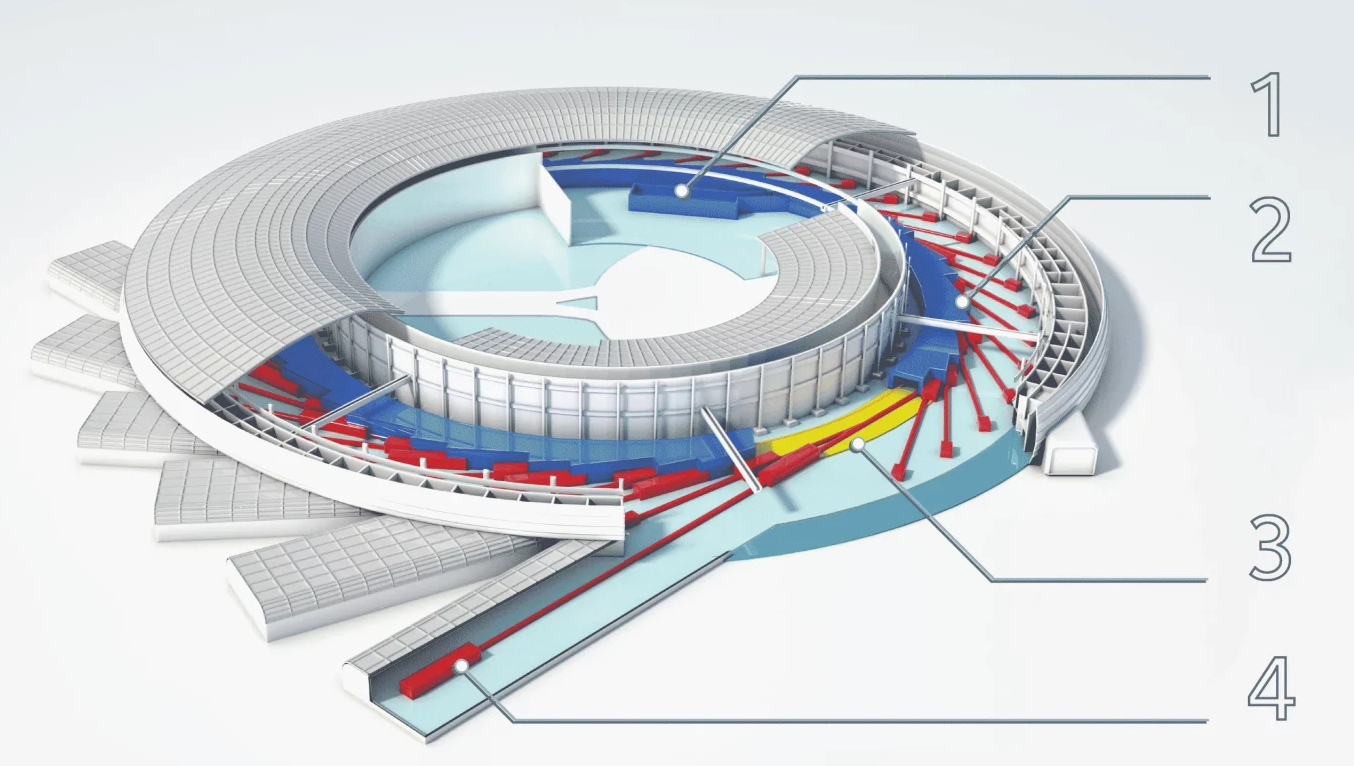
\includegraphics[width=0.8\textwidth]{Images/sirius_facility.png}
    \caption{Schematic view of the SIRIUS installations. 1) Linear accelerator (LINAC); 2) Concrete tunnel housing the booster accelerator and the storage ring; 3) storage ring; 4) beamlines. From \href{https://lnls.cnpem.br/sirius/como-funciona-o-sirius/}{LNLS website}.}
    \label{fig:sirius_layout}
\end{figure}
\subsubsection{Storage ring magnets and RF cavity}
\begin{figure}[tb]
    \centering
    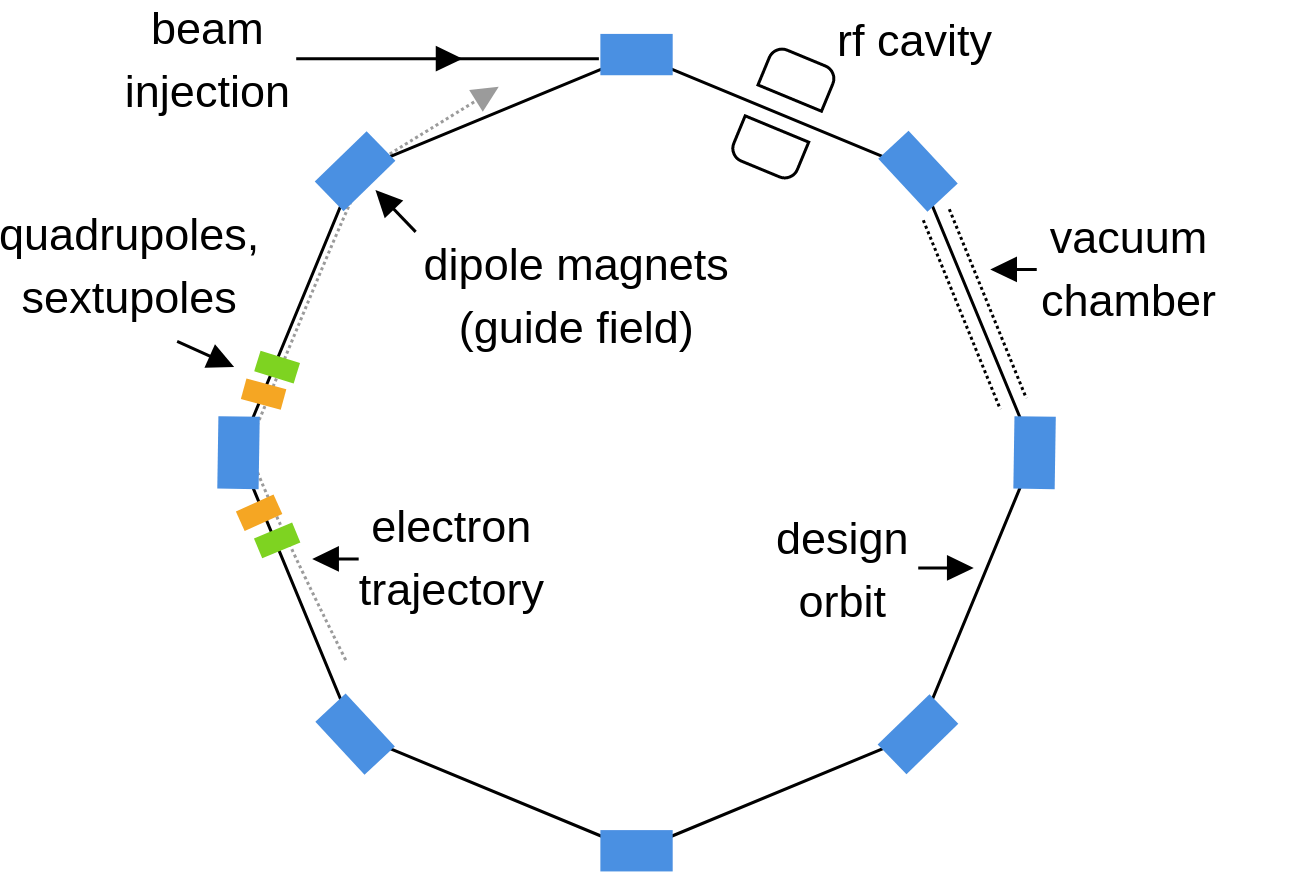
\includegraphics[width=0.4\textwidth]{Images/storage_ring.png}
    \caption{Storage ring typycal configuration. From \cite{sands_1969}}
    \label{fig:storage_ring}
\end{figure}
\todo[inline]{draw my onw figure}
Figure~\ref{fig:storage_ring} sketches the typical layout of a syncrhotron accelerator. The electron beam is stored within a vaccum chamber, oscillatin in proximity to a reference design closed orbit under the influence of an array of magnets. The orbit is determined by the strengths of the deflection magnets, the dipoles, and the operation energy of the beams. A pure dipole magnet provides an uniform and homogeneous magnetic field perpendicular to the facility floor and bends the electrons trajectory in the direction parallel to the floor. For the trajctories resulting in a closed orbit, the overall bending angle provided by the dipoles along the entire ring must equal $2\pi$ radians. The field profile of a dipole magnet is depicted in the left side sketch of Fig.~\ref{fig:magnets_fields}. Imagining a beam directed inward the screen, the trajectory will be bent to the right.

To maintain electrons in close proximity to the reference orbit, focusing of the trajectories is required. Focusing is attained by employing gradient fields, primarily generated by quadrupole magnets at SIRIUS. The strength of such fields increase linearly with deviations from the closed orbit, which lies in the magnet's center. Gradient fields effectively act as spring forces. The mangets poles and the field profile of a quadrupole magnet are depicted in the center sketch of Fig.~\ref{fig:magnets_fields}.

Focusing and deflection are energy-dependent, which means small deviations from the nominal operating energy can result in differential focusing. Drawing an analogy from geometric optics, the beam's focusing behavior at the "lens" (quadrupoles) depends on its "color" (energy). To correct for these chromatic aberrations, the use of "glasses" becomes necessary. In the context of accelerators, sextupole fields serve as these corrective lenses. They introduce geometric aberrations to counteract the chromatic ones, resulting in approximately uniform, energy-independent focusing, up to the linear approximation theory. The mangets poles and the field profile of a sextupole magnet are depicted in the right sketch of Fig.~\ref{fig:magnets_fields}.
\begin{figure}[htb]
    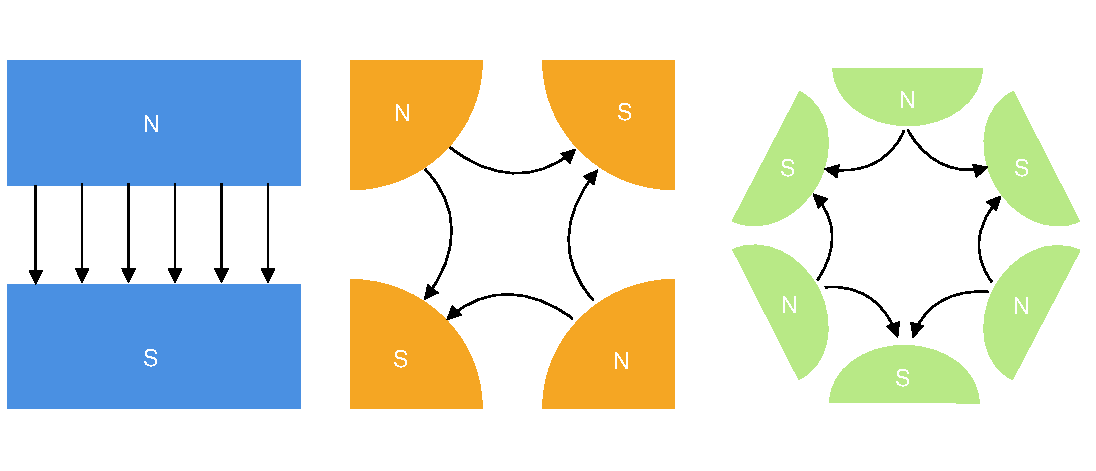
\includegraphics[width=\textwidth]{Images/magnets.pdf}
    \caption{Schematic representation of the magnets comprising SIRIUS lattice and their fields profile. From left to right: dipole magnet, quadrupole magnet and sextupole magnet.}
    \label{fig:magnets_fields}
\end{figure}

Besides dipoles, quadrupoles and sextupoles, additional dipole actuators magnets for orbit/trajectory correction and pulsed magnets for beam injection are also part of the ring. The beam is also periodically subject to longitudinal time-dependent electromagnetic radiofrequency fields which do work on the beam to replenish its energy. The goal is to compensate for the energy carried away in the form of synchrotron light.

\section{The problem addressed in this work}
The pursuit of low emittances and high brightness has driven the accelerator community toward the fourth-generation of storage rings. Achieving such low emittances was possible because of series of technological advances which enabled the use of the multi-bend achromat (MBA) lattice\cite{liu_towards_2017,hettel_challenges_2014}. MBA lattices require intense gradient fields provided by quadrupole magnets, which, in turn, demands the presence of strong sextupolar fields to compensate for chromatic effects. Since sextupoles provide nonlinear fields, the dynamics in fourth-generation storage rings has become increasingly nonlinear\cite{liu_towards_2017}.

A quasi-periodic nonlinear dynamics, when subjected to even the slightest perturbations—such as small field errors stemming from rotation, alignment, or fields excitation errors—can potentially become unstable at large oscillation amplitudes. These instabilities impose constraints on the maximum transverse oscillation amplitudes that the machine can accommodate. The specific amplitude below which motion is stable is referred to as the Dynamic Aperture (DA) of the ring. Exceeding the DA results in irregular and often chaotic motion and beam loss.

Under normal operating conditions, the equilibrium beam size and typical oscillation amplitudes are considerably smaller than the DA, and the dynamics can be well studied and analyzed using a linear approximation theory, without worrying about the DA. However, there are specific scenarios where the DA becomes crucial for the operation, notably during the injection process.

During injection into the storage ring for beam accumulation, the beam is extracted from the booster accelerator and guided toward the storage ring through a transport line. As soon as it enters the ring, the beam is deflected by the field of a pulsed nonlinear magnet, which makes the beam almost parallel to the storage ring tangent direction, albeit with a horizontal offset of approximately $x=-8~\unit{mm}$ \cite{liu_injection_2016}. If the DA is smaller than this initial amplitude, it imposes limitations on the injection efficiency.

The placement, symmetry and strength of sextupoles magnets--the nonlinear lattice-- were determined through a multi-objective optimization process, primarily focused on improving the simulated DA and beam lifetime of the machine's computer model\cite{de_sa_optimization_2016, dester_energy_2017}. This optimization work considered the average performance of the lattice configurations while accounting for various magnet errors that simulate the expected errors in the actual machine \cite{de_sa_optimization_2016}. Several models, with several errors distribution among the magnets were generated, and the DA and lifetime for a given lattice configuration was calculated by simulating the electron beams motion for several turns (tracking simulations). The final figure of merit for a lattice consisted on the average DA and lifetime it provided to the ensemble of machines. The best-performing machine lattice found during this process was adopted as the nominal lattice which was subsequently deployed during the commissioning phase of the machine.

The operating machine consists on a practical realization of a specific error configuration, which defines the physically realized magnetic lattice and determines the dynamics overall performance. The best-performing lattice on average, found in the simulations, is not necessarily the optimum lattice for this specific errors realization.

Assuming the realized lattice closely approximates the optimum setup, i.e. that the errors are small, it is reasonable to assume that by making minor tweaks and adjustments to the strengths of the sextupoles one can adapt the nonlinear lattice to match the actual distribution of errors in the physical system. This fine-tuning process can result in improved nonlinear dynamics performance, expanding the DA, and ultimately enhancing both injection efficiency and its stability. This process has already been demostraded in other machines. It has proven to be a succesfull approach and became knonw as \textit{Online optimization}. If one thinks of the errors as agents that deteriorate the DA from its optimum, online optimization can be seen as an attempt to compensate for such deterioration.

Online optimization of the machine nonlinear dynamics consists on employing computer-automated search strategies to systematically explore various sextupole configurations with the goal of identifying the ones that yields the largest DA while not interfering in other machine parameters, such as chromaticity and beam lifetime. The key ingredient in online optimization is the choice of a robust optmization algorithm based on direct or indirect search in the parameter space. The most widely used is the Robust Conjugate Direction Search (RCDS) algorithm, which is based on a noise robust one-dimensional optimizer along with a clever strategy, known as Powell's method, for choosing directions in the search space. Chapter 3 addresses the RCDS algorithm.

Besides improving the DA and injection efficiency in nominal operation conditions, it is also interesting to do so in different machine \textit{working points}, with different \textit{tunes}. As chapter 2 shows, if one fixes one's attention to a specific point of the ring, and measure the beam position in horizontal and vertical planes for consecutive turns, one realizes the motion is a sampled sinusoid and the tunes $\nu_x$ and $\nu_y$ are the fundamental frequencies of such harmonic motion. They are important operation parameters  since they affect over the response of the system in the presence of pertrubations. Tunes close to integer numbers result in large \textit{orbit amplification factors} making the dynamics particularly sensitive to perturbations.

The fractional parts of SIRIUS nominal tunes are quite low and increasing them would distance the tunes away from integer numbers, reducing the orbit amplification factors and improving the orbit stability. Changing the tunes can be achieved by actuating with the quadrupole magnets, but doing so takes the machine to a different operating optics, in which the DA can, and often is, smaller than the DA in nominal optics. In different working points, thus, online optimization is essential to find a new sextupole configuration to adapt the nonlinear mangets to the new optics and  achieve a good DA and acceptable injection efficiencies for operation.

In agreement with the experience in other facilities, it is shown in Chapter 4 that online optimization using RCDS can succesfully improve the dynamics performance and lead to DA and injection efficiency improvements. This was observed for the SIRIUS storage ring both in the machine nominal tunes as well as in other working points.  SIRIUS experience with online optimzation is a valuable demonstration of this tool's efficiency in fourth-generation rings with such a large search space.

At the time of this writing, SIRIUS is operating with the sextupole configurations found during one of the experiments carried out during the execution of this project. The configuration was found by online optimzination carried out with increased tunes optics. The higher tunes led a reduction in obrit amplification factors resulting in unprecedent orbit stability.

In the next chapter, the dynamics of electrons in storage rings is examined. The linear approximation motion is introduced and nonlinear dynamics is trated as a perturbation to the linear theory. Chapter 3 gives the reader a brief overview of optimization strategies and focuses on familiarizing the reader with the Robust Conjugate Direction Search (RCDS) algorithm. Chapter 4 presents the methods and results of the online optimization experiments carried during the execution of this project.
